\chapter{Програмна реализация на система за прогнозиране}

На база на разгледаните алгоритми и системи за прогнозиране, изборът за изработка на софтуерна система за прогнозиране пада върху клиент-сървър базирана архитектура, в която мобилни устройства извършват изчисления на изчислими пакети. Изчисленията се организират под формата на дарена изчислителна мощност. 

\section{Архитектура на системата}

Най-обобщеното представяне на разработената система съдържа трите най-важни компонента – сървър, комуникационна среда и мобилни устройства (Фиг. \ref{fig0054}). Комуникационната среда е глобалната мрежа Интернет. Информацията, която трябва да бъде изчислена, основно се намира на специално предназначен за нуждите на системата сървър. Изчислителните възли в системата са умни мобилни устройства. 

Основна цел при разработването е крайното решение да бъде максимално икономически изгодно. Това означава, че разходите за поддържане на цялата инфраструктура трябва да бъдат минимизирани. Тази цел може да бъде постигната, ако разходите за поддържането на сървър бъдат снижени възможно най-много. Системата трябва да работи с маломощен сървър, който само да синхронизира пресмятанията и да съхранява получените междинни резултати. Тъй като потребителите в системата даряват техните изчислителни ресурси, практически разходите от страна на клиента са сведени до нула. Всеки потребител сам закупува мобилното си устройство, сам заплаща сметката за изразходвания Интернет трафик и сам заплаща електричеството, необходимо за опериране на устройството. Поради стремежа за минимално натоварен сървър, вместо закупуването на отделна сървър машина и разполагането й в информационен център, спокойно може да се наеме уеб услуга от тип споделен хостинг (Фиг. \ref{fig0055}). 

\begin{figure}[H]
  \centering
  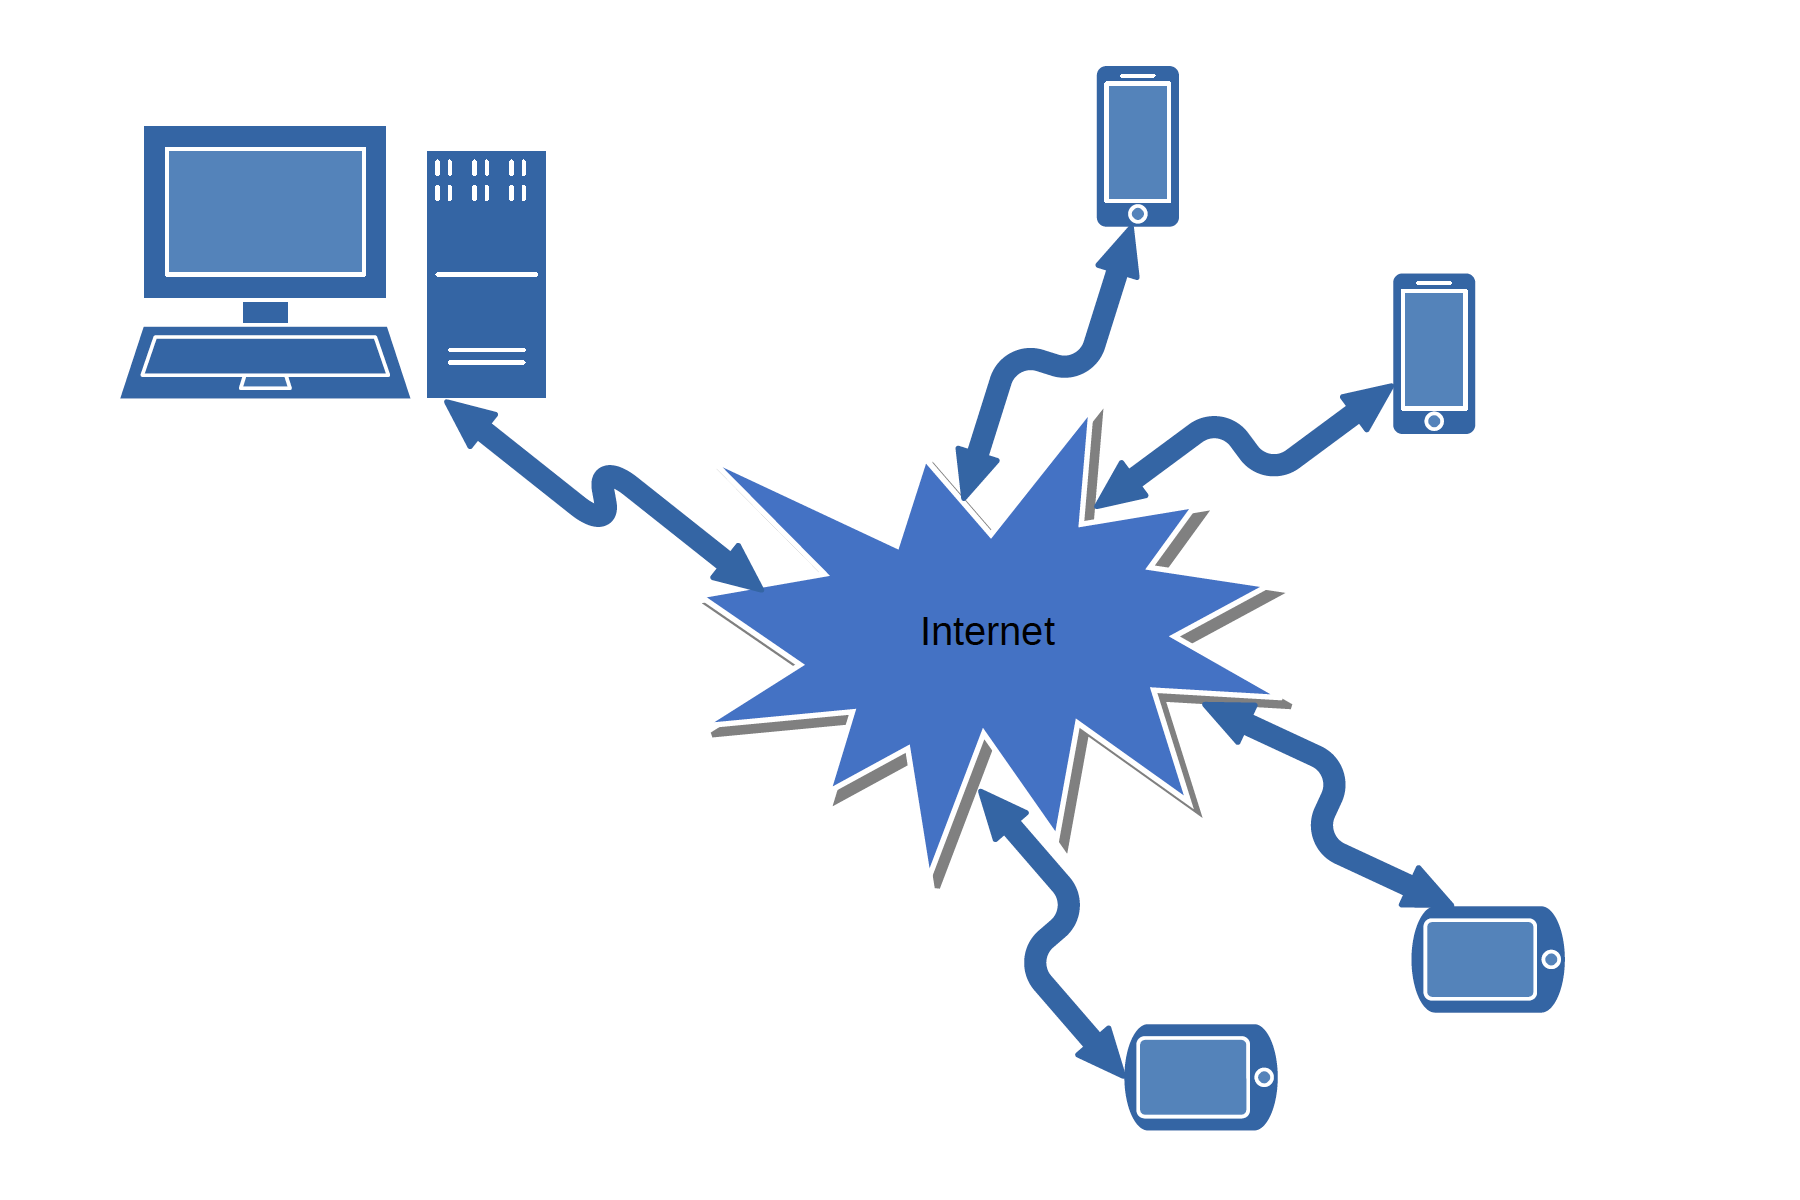
\includegraphics[width=0.8\linewidth]{fig0054.png}
  \caption{Обща организация на системата}
\label{fig0054}
\end{figure}

При споделения хостинг, върху една физическа машина доставчикът стартира множество виртуални машини и в самите виртуални машини се активират отделни инстанции на уеб сървърни приложения. Най-често използваните от доставчиците на споделен уеб хостинг операционни системи са базирани на Linux. Операционната система Linux много добре се съчетава с уеб сървъра Apache. Към уеб сървъра доставчиците най-често предлагат и MySQL релационна база данни. Apache уеб сървъра най-често има настроена поддръжка на PHP интерпретатора. Споделен хостинг в конфигурация Linux-Apache-MySQL-PHP (XAMPP) е едно от икономически най-ефективните решения. Като алтернативи може да се ползват Windows базирани сървъри, който поддържат MS SQL Serve база данни и ASP.NET уеб страници. Възможни са също комбинации с JSP, PostgreSQL или Oracle, но никоя от изброените комбинации не може да постигне икономическата ефективност на XAMPP. Споделеният хостинг при конфигурация XAMPP може да се наеме за абонамент от няколко долара на месец. 

\begin{figure}[H]
  \centering
  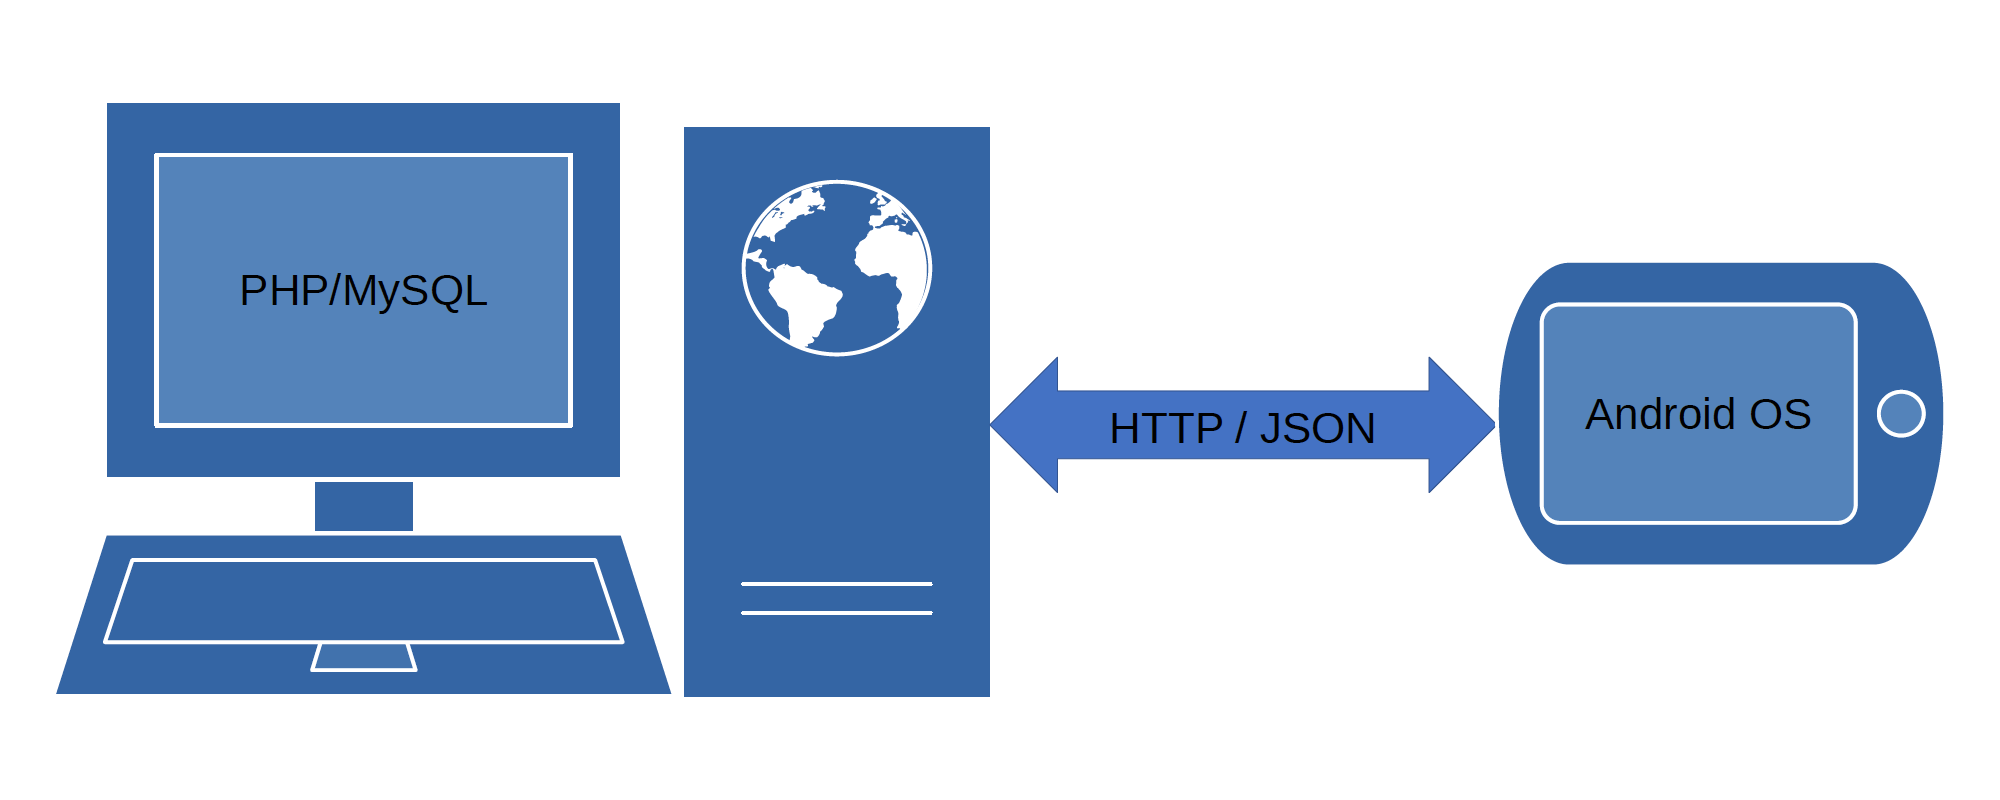
\includegraphics[width=0.8\linewidth]{fig0055.png}
  \caption{Софтуерни компоненти}
\label{fig0055}
\end{figure}

Комуникацията в системата винаги се инициира от клиентското приложение, което отправя заявки към сървъра и връща резултати. Комуникацията се извършва по протокола TCP/IP, като се използват възможностите за HTTP комуникация. По аналогия с RESTful приложенията, клиентът и сървърът обменят съобщения пакетирани с JSON. Ролята на JSON е в това информацията да бъде предавана по мрежата в структуриран вид. Възможна е реализация и с XML, но JSON е значително по-добре оптимизиран за комуникация между машини. XML намира по-широко приложение там където е нужна човешка намеса за описване на данните. JSON има и предимството, че обемът служебна информация е значително по-малък в сравнение с XML. 

От страната на клиента, стои Android OS приложение, разработено към настоящия дисертационен труд, което има основната задача да извършва разпределените изчисления и да докладва получените резултати на отдалечения сървър. Сървърното приложение не е част от настоящия дисертационен труд, а се използва на база на предходна разработка в ИИКТ-БАН \cite{Balabanov-04}. 

Изборът на мобилни устройства с операционна система Android OS е направен, тъй като тези устройства са много разпространени, със значителен пазарен дял, ядрото на операционната система е Linux базирано, а множество нейни компоненти са с отворен код. От значение е и цената на мобилните устройства, тъй като прекият конкурент iOS, на компанията Apple, поддържа значително по-високи цени. При дарените ресурси за разпределени изчисления е от съществено значение крайните потребители да могат да си позволят цената на изчислителните ресурси. Сериозно предимство на Android OS е и факта, че поддържа програмния език Java. По настояще, Java е най-широко използвания програмен език, което го прави изключително подходящ от гледна точка на човешки ресурси, при евентуално разрастване на проекта. В последните години се забелязва много силно наложена тенденция езикът Java да бъде подменен в Android OS с езика Kotlin, но този процес би отнел твърде много време. Предимство на програмния език Java е и това, че той широко се използва не само за програмиране на мобилни приложения, но и на множество други видове софтуер. За сравнение, езиците Objective-C и Swift, на компанията Apple, далеч не се използват толкова много, извън продуктите на самата компания. Това ограничение би довело до сериозни проблеми при търсенето на програмисти за мобилни устройства базирани на операционната система iOS. 

\section{Модулна организация на мобилното приложение}

Разработката на мобилното приложение е организирана в отделни модули. Използването на модули позволява по-гъвкава работа с различните компоненти и по-лесно тестване на написания програмен код. Модулността позволява отделни части от приложението да се използват по различен начин. На най-високото ниво за разделяне са налични три модула – изчислителен модул, Android OS потребителски интерфейс и интерфейс за терминален прозорец на настолна операционна система (Фиг. \ref{fig0056}).

\begin{figure}[H]
  \centering
  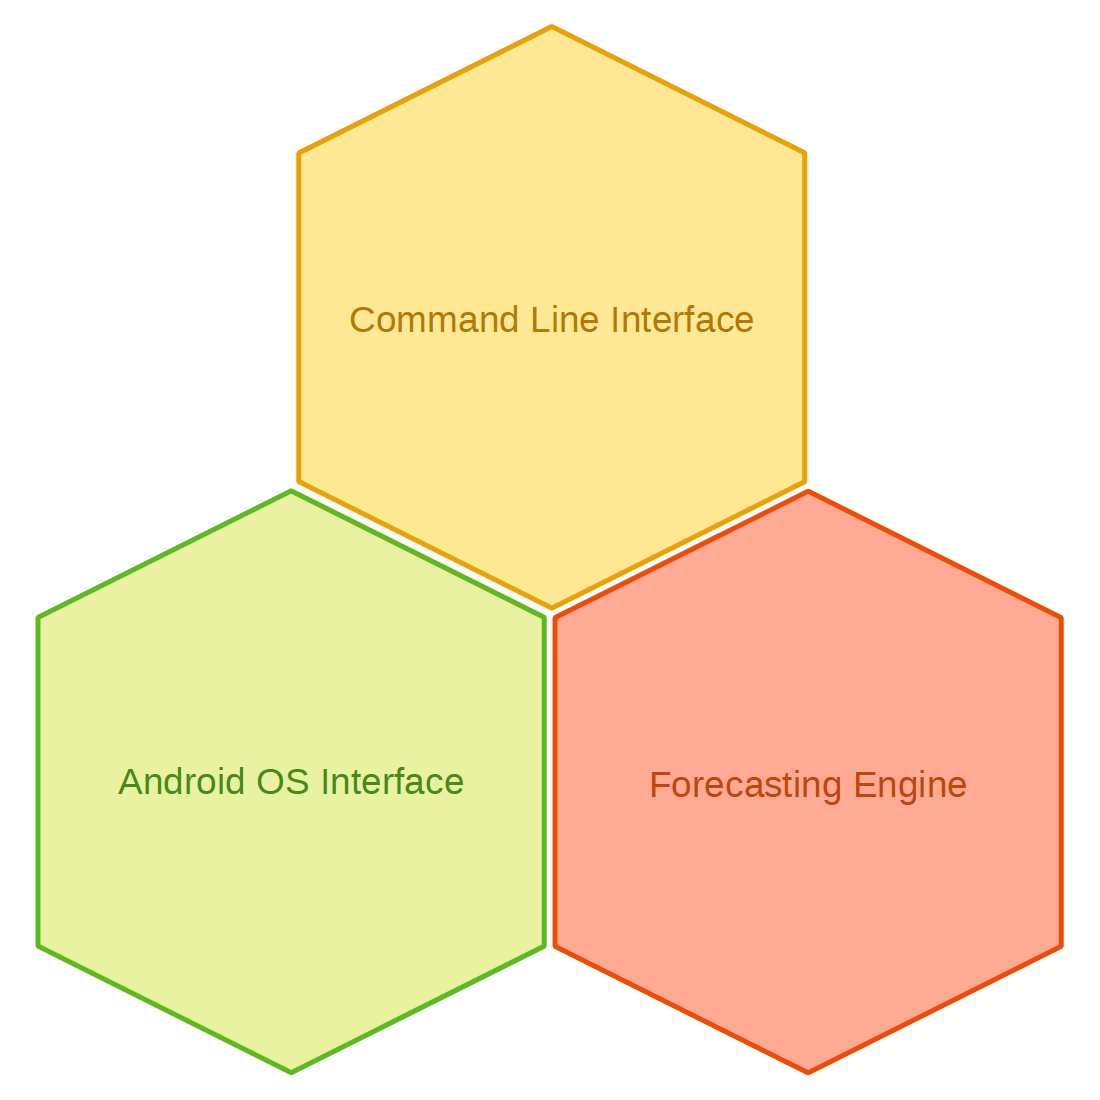
\includegraphics[width=0.8\linewidth]{fig0056.png}
  \caption{Основни модули на мобилното приложение}
\label{fig0056}
\end{figure}

Всички съществени пресмятания се реализират в изчислителния модул. Стремежът в този модул е той да не използва специфичен код от API-то на Android OS или на някоя от операционните системи за настолни компютри. Целта на това разделяне е изчислителният модул да има своята самостоятелност и с лекота да се вгражда в модули се интегрира в модули за графичен потребителски интерфейс или интерфейс от тип команден ред. 

Модулът реализиращ интерфейс в командния интерпретатор е полезен при изпитанията на системата, тъй като с него може да се избегне времеемкото зареждане на Android приложение в Android емулатор. Модулът за команден интерпретатор се компилира със стандартните развойни средства на Java, до самостоятелно приложение за настолен компютър. Този начин на работа улеснява търсенето на дефекти, когато съмненията са в начина на работа на Android OS интерфейса и изчислителния модул. 

Модулът за графичен потребителски интерфейс на Android OS има основна задача да извършва пресмятанията на фонов режим (Android Services). Също така, този модул визуализира информацията за междинните резултати от пресмятанията. Модулът извършва съхраняването и зареждането на локалната информация в SQLite релационна база данни. Дава и възможности за настройки за начина по който функционира мобилното приложение. 

\subsection{Компоненти в модула за графичен интерфейс}

Комуникацията на Android OS с компонентите на модула за графичен интерфейс става през няколко компонента. В Android е възприета концепцията на уеб страниците, където няма единична точка за стартиране на приложението, а различните компоненти могат да бъдат извикани по отделно, точно както може да се отворят различни страници, а не задължително заглавната страница. 

\begin{figure}[H]
  \centering
  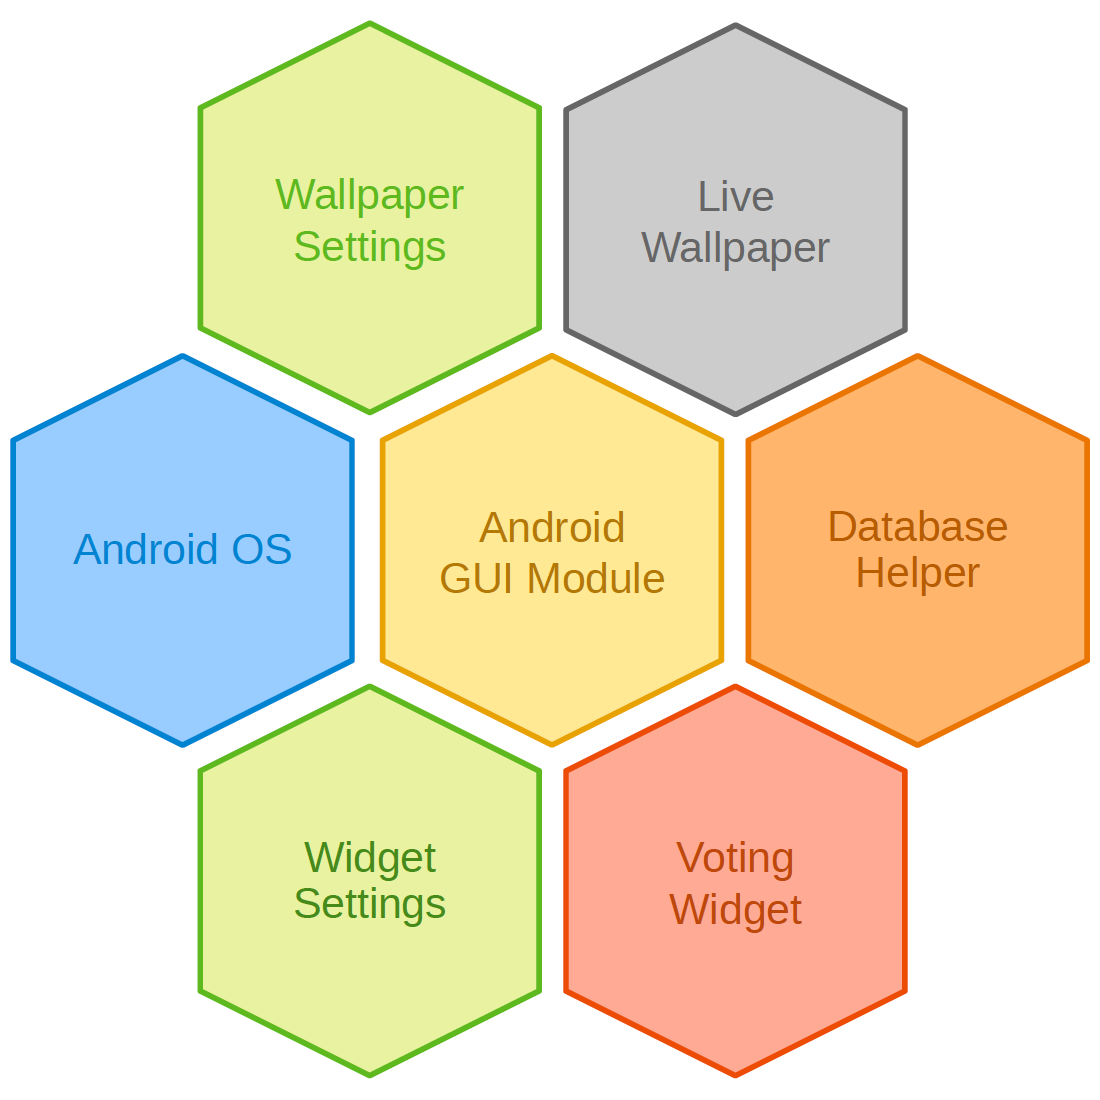
\includegraphics[width=0.8\linewidth]{fig0057.png}
  \caption{Компоненти в GUI модула}
\label{fig0057}
\end{figure}

На този етап от завършеността на системата, активният тапет е основният компонент на мобилното приложение. Активните тапети задават фоново изображение, което стои зад всички компоненти на работния плот (Фиг. \ref{fig0058}). Тапетите са активни, защото по своята същност не са статично изображение, а цялостна работеща програма, която позволява динамично изрисуване в растерно платно. Активният тапет се управлява от операционната система чрез услуга/демон (Android Services). Услугите в Android са програми, които не притежават свой собствен потребителски интерфейс. Услугите са аналог на демон процесите в операционните системи за настолни компютри. 

\begin{figure}[H]
  \centering
  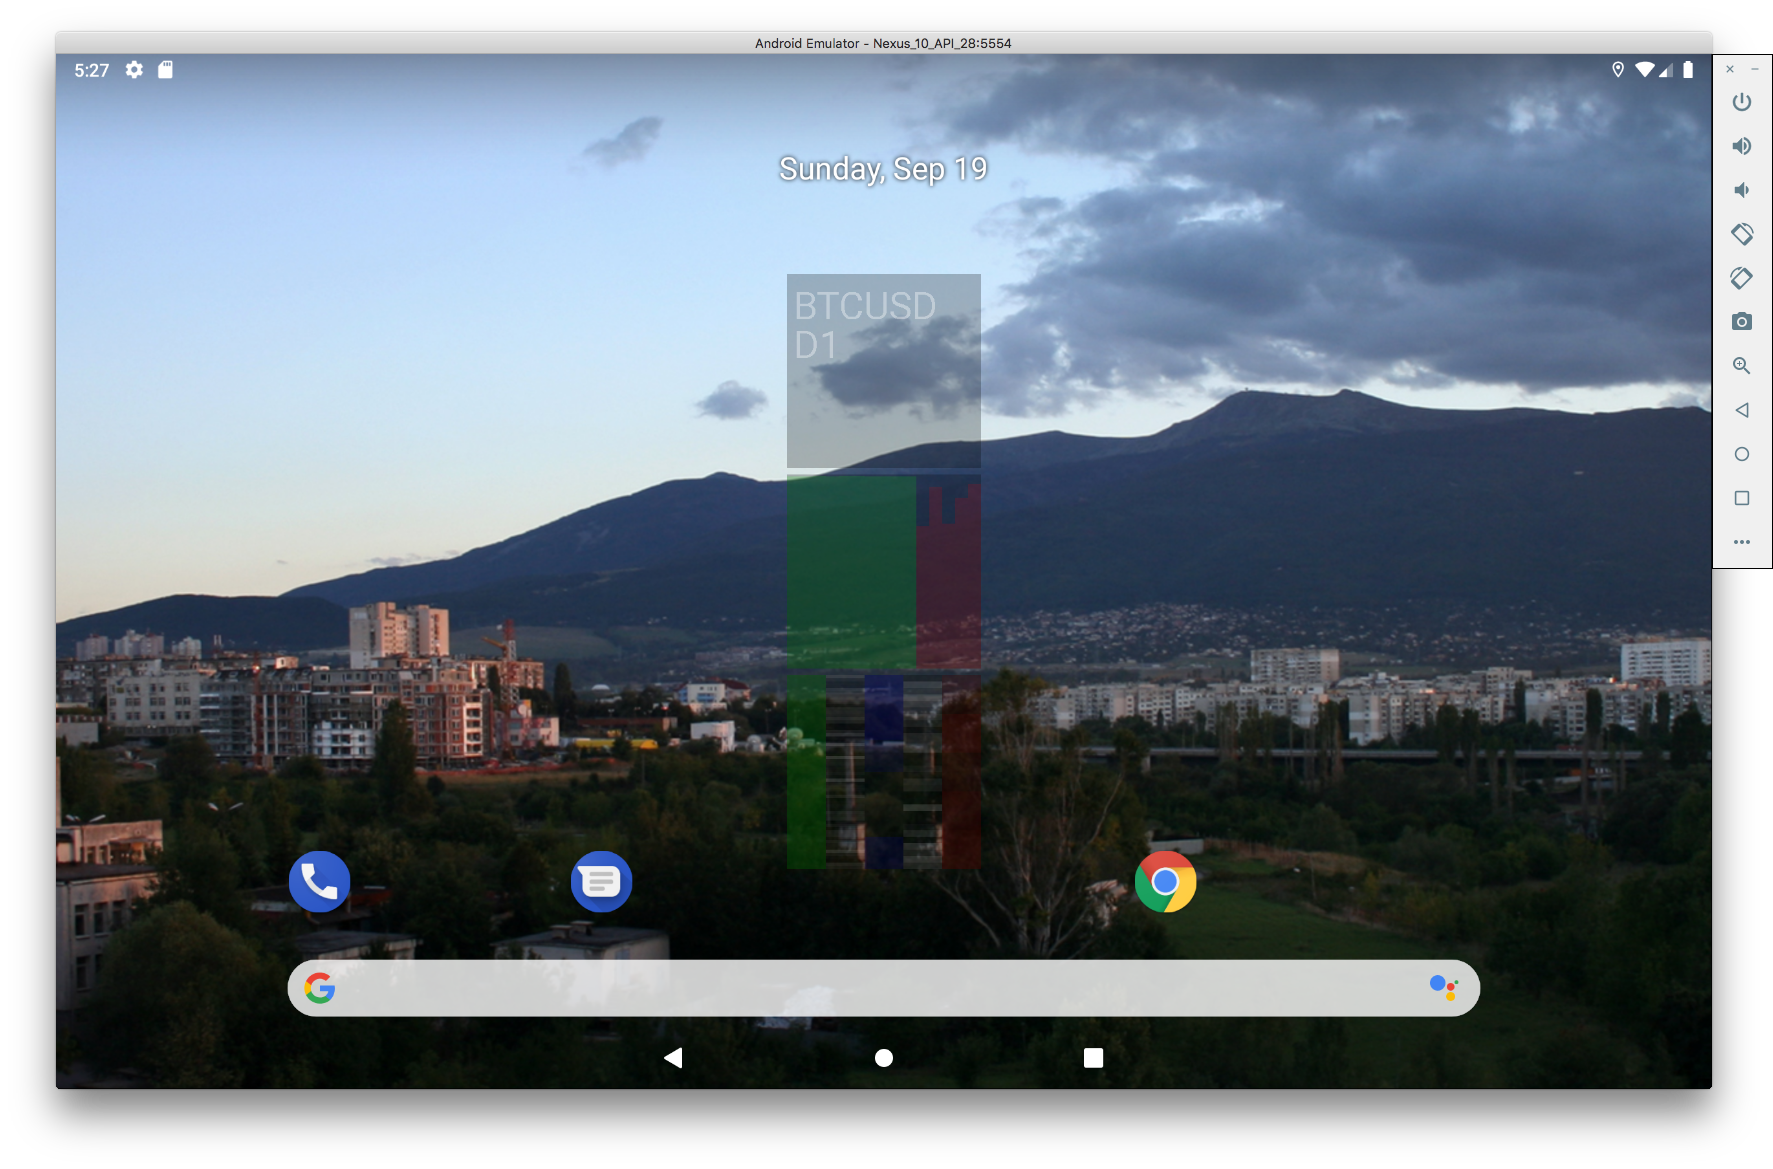
\includegraphics[width=0.8\linewidth]{fig0058.png}
  \caption{Android Live Wallpaper}
\label{fig0058}
\end{figure}

Тъй като използването на устройството във фонов режим, за извършване на изчисления може да забави сериозно работата му, то активният тапет разполага с екран за настройки (Фиг. \ref{fig0059}). В този екран се определя честотата за извършване на пресмятания, както и някои опции свързани с визуализацията на междинните резултати. 

\begin{figure}[H]
  \centering
  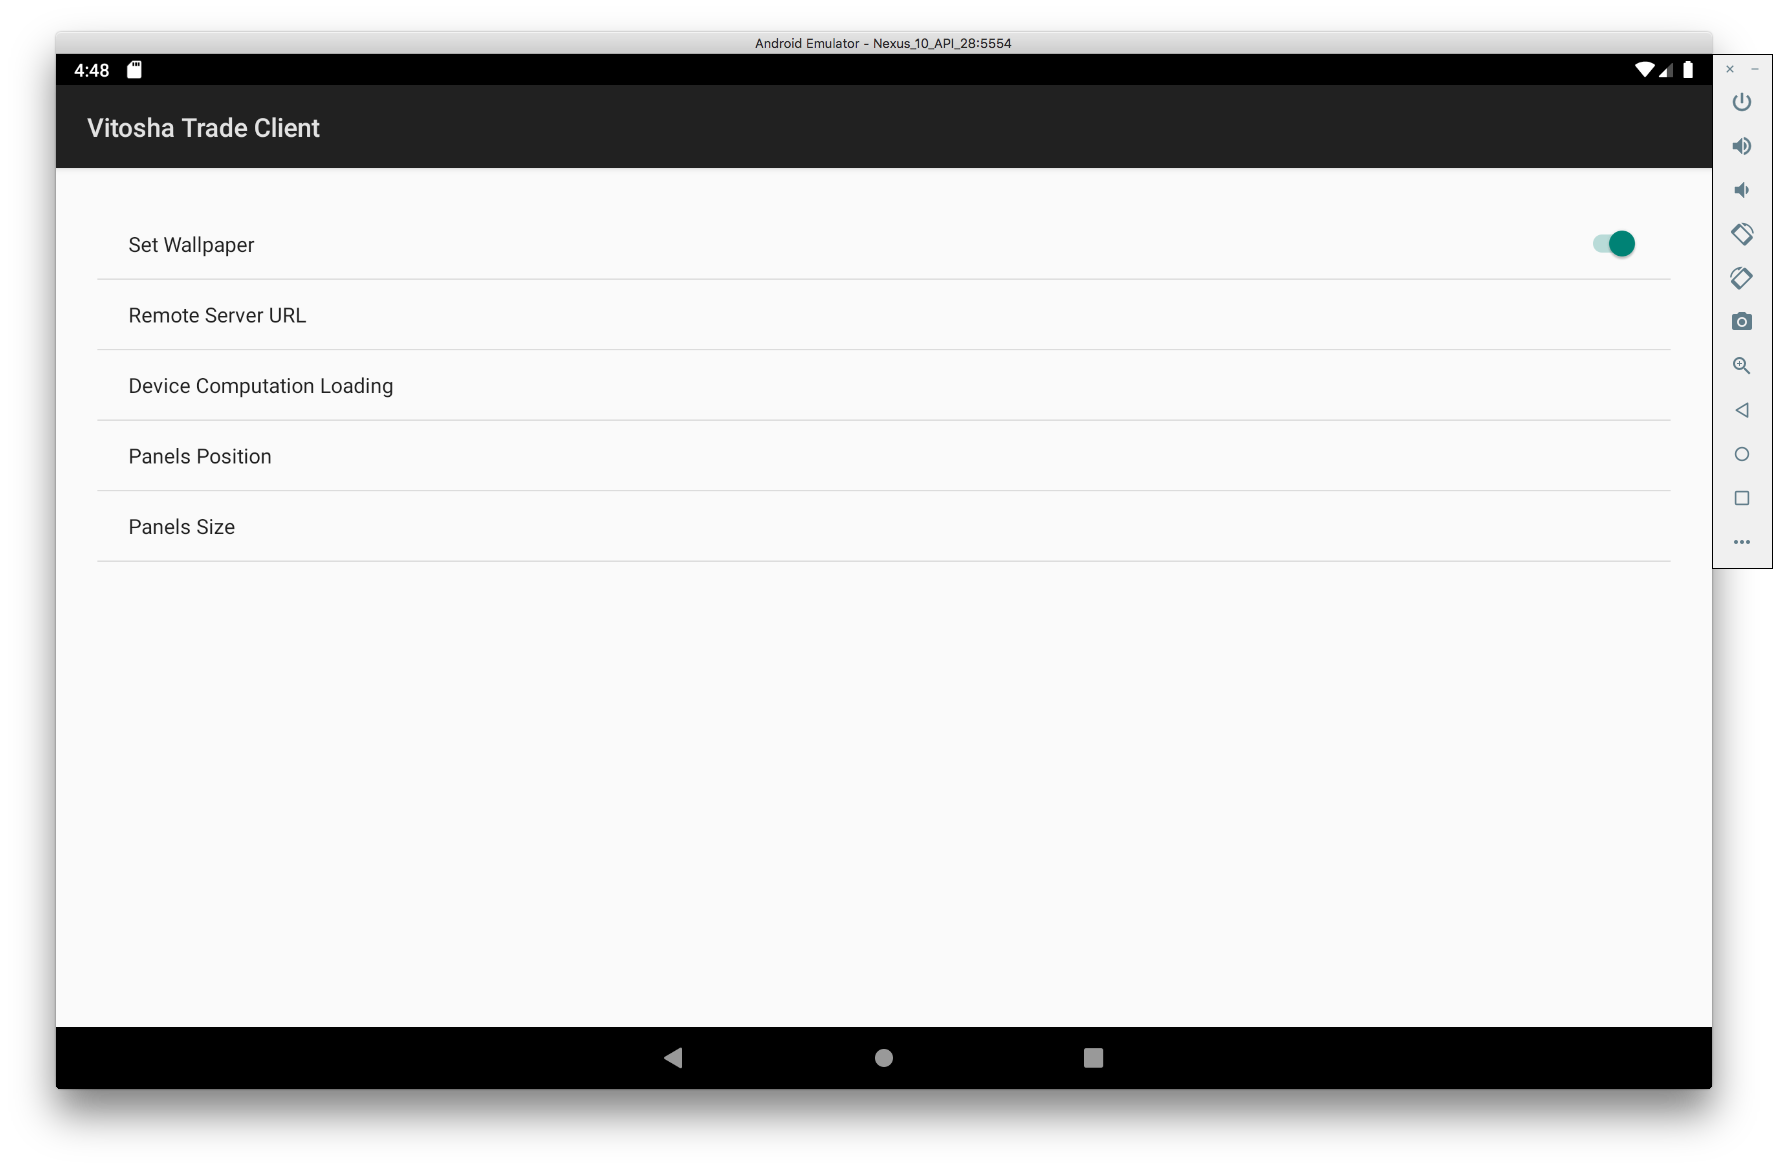
\includegraphics[width=0.8\linewidth]{fig0059.png}
  \caption{Настройки на активния тапет}
\label{fig0059}
\end{figure}

Цялата информация за извършване на изчисленията върху мобилното устройство се получава от отдалечен сървър на конкретно установен URL адрес (Фиг. \ref{fig0060}). Натоварването на мобилното устройство е организирано в пет възможни степени (Фиг. \ref{fig0061}). Позициите на панелите за визуализация на междинната информация се определя от списък с възможности (Фиг. \ref{fig0062}). Размерите на панелите за визуализация са ограничени в три опции (Фиг. \ref{fig0063}).

\begin{figure}[H]
  \centering
  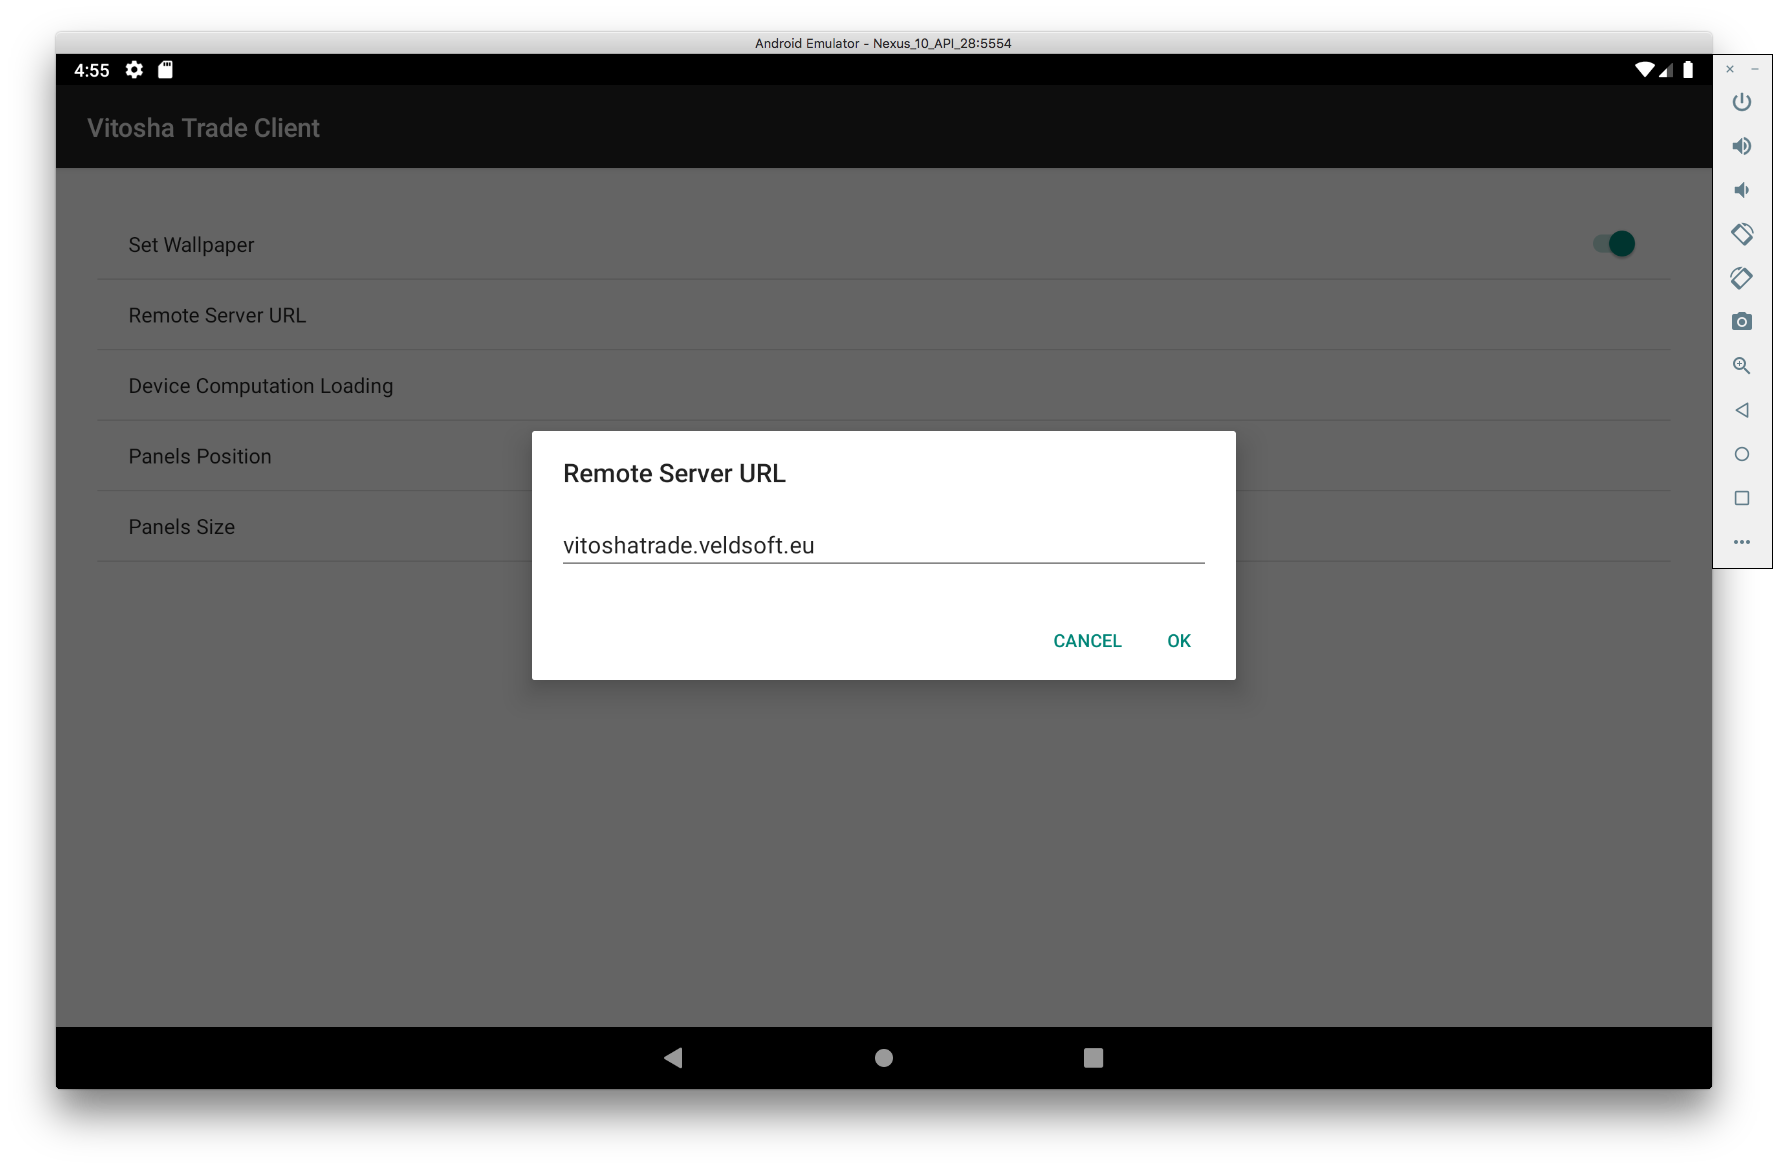
\includegraphics[width=0.8\linewidth]{fig0060.png}
  \caption{Адрес на отдалечения сървър}
\label{fig0060}
\end{figure}

Адресът на отдалечения сървър представлява буквено-символно име, което води към компютър, който изпълнява приложение за уеб сървър и поддържа нужните скриптове за JSON обмен на съобщения с клиентското приложение.

\begin{figure}[H]
  \centering
  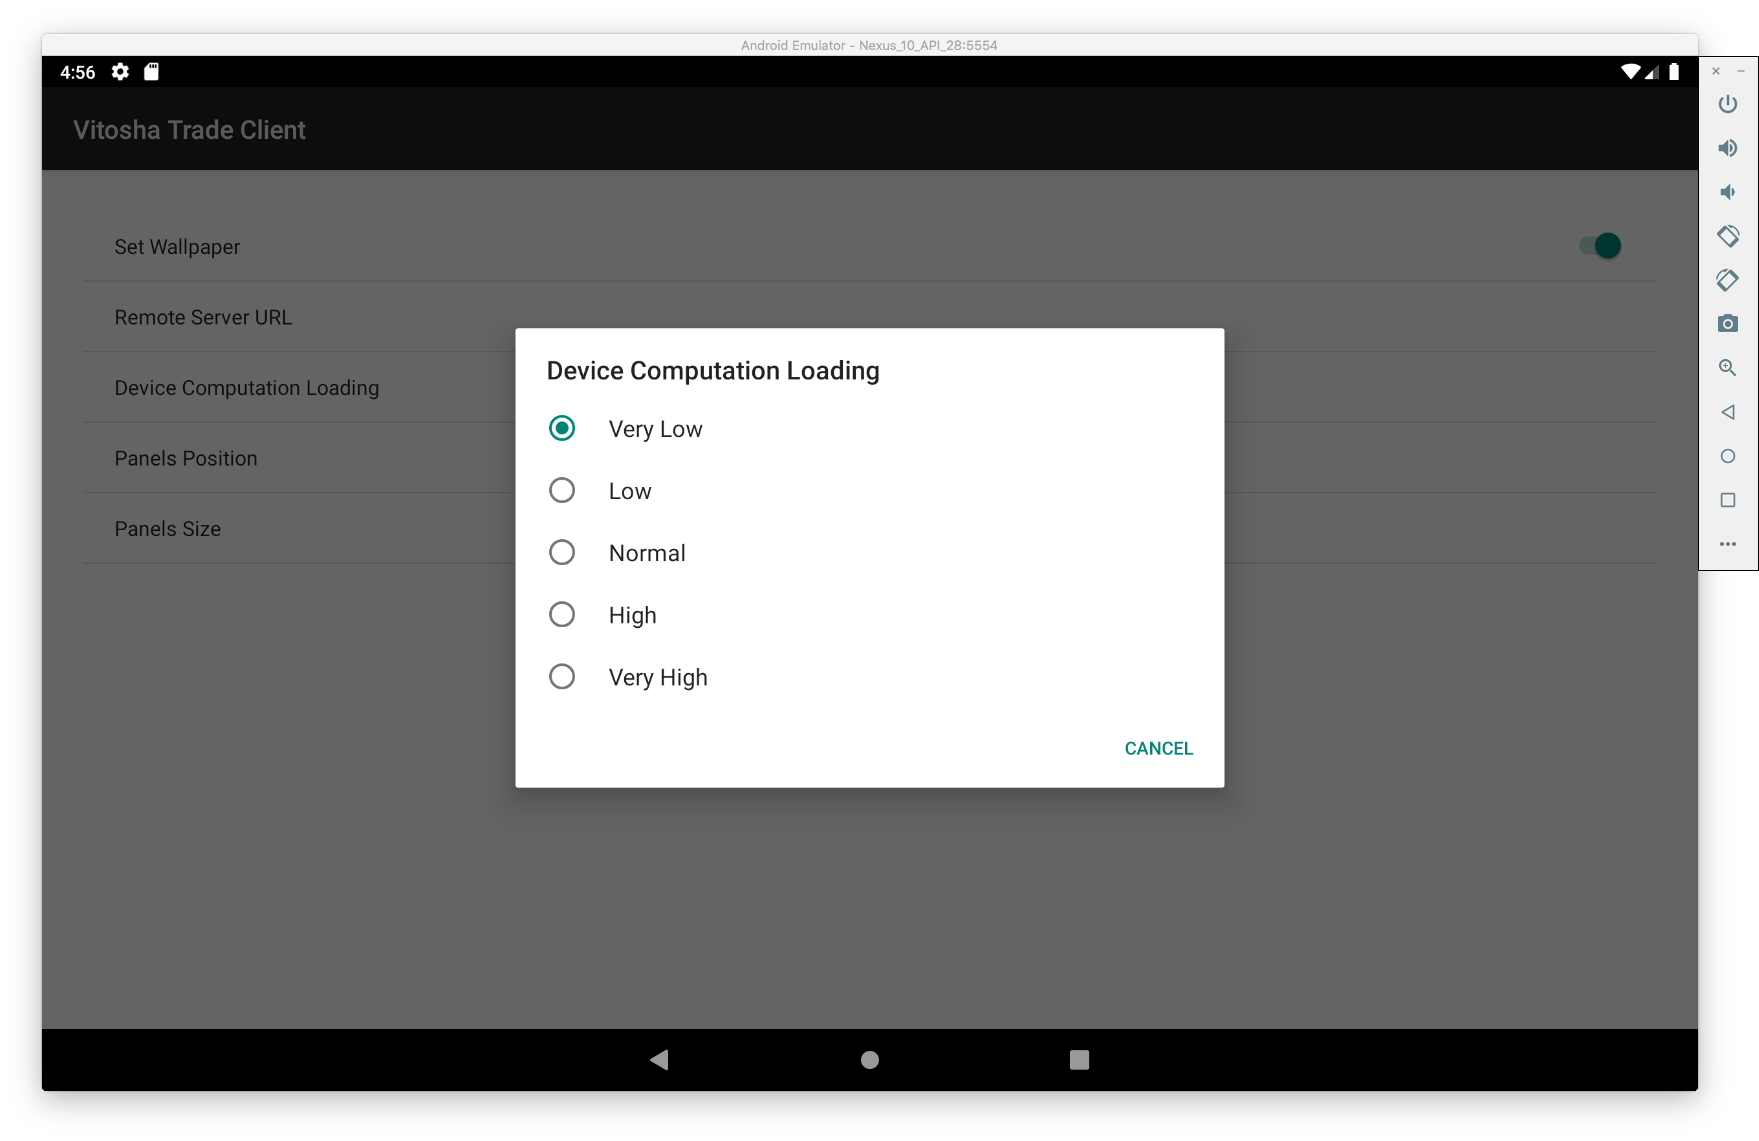
\includegraphics[width=0.8\linewidth]{fig0061.png}
  \caption{Натоварване на мобилното устройство}
\label{fig0061}
\end{figure}

Натоварването на мобилното устройство се регулира с период през който да се стартира единичен цикъл за обучение и прогнозиране. Твърде дългите интервали забавят процеса на смятане, но разтоварват мобилното устройство от консумация на енергия и забавяне на общата производителност.

\begin{figure}[H]
  \centering
  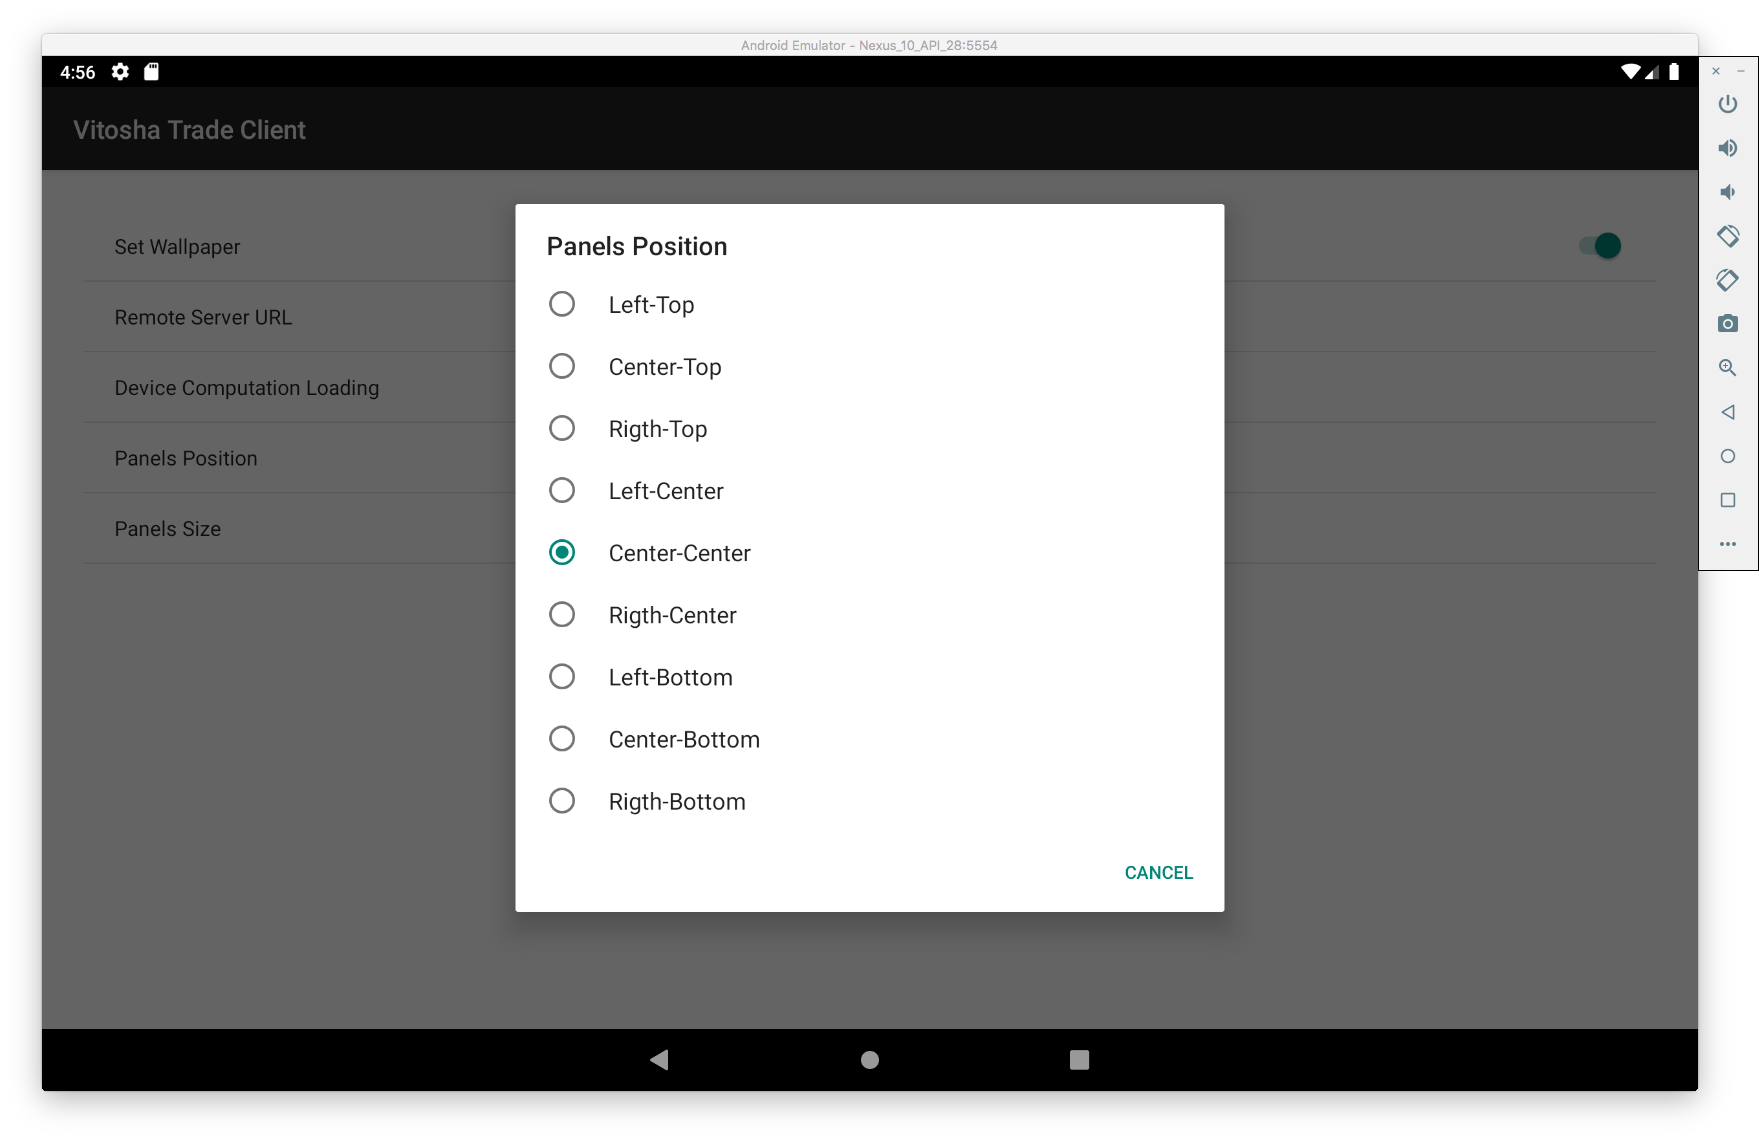
\includegraphics[width=0.8\linewidth]{fig0062.png}
  \caption{Позиция на панелите за визуализация}
\label{fig0062}
\end{figure}

Според организацията на работния плот, всеки потребител има различни предпочитания в коя част на екрана му е удобно да получава фонова визуална информация. Чрез възможността за промяна на позициите, панелите за визуализация могат да са максимално информативни за потребителя. Разликата в размерите на различните екрани води до допълнителна необходимост за размерите на панелите за визуализация. При устройства с големи екрани е рационално панелите да са по-големи, а при устройства с малки екрани е рационално панелите да са с по-малки размери. 

\begin{figure}[H]
  \centering
  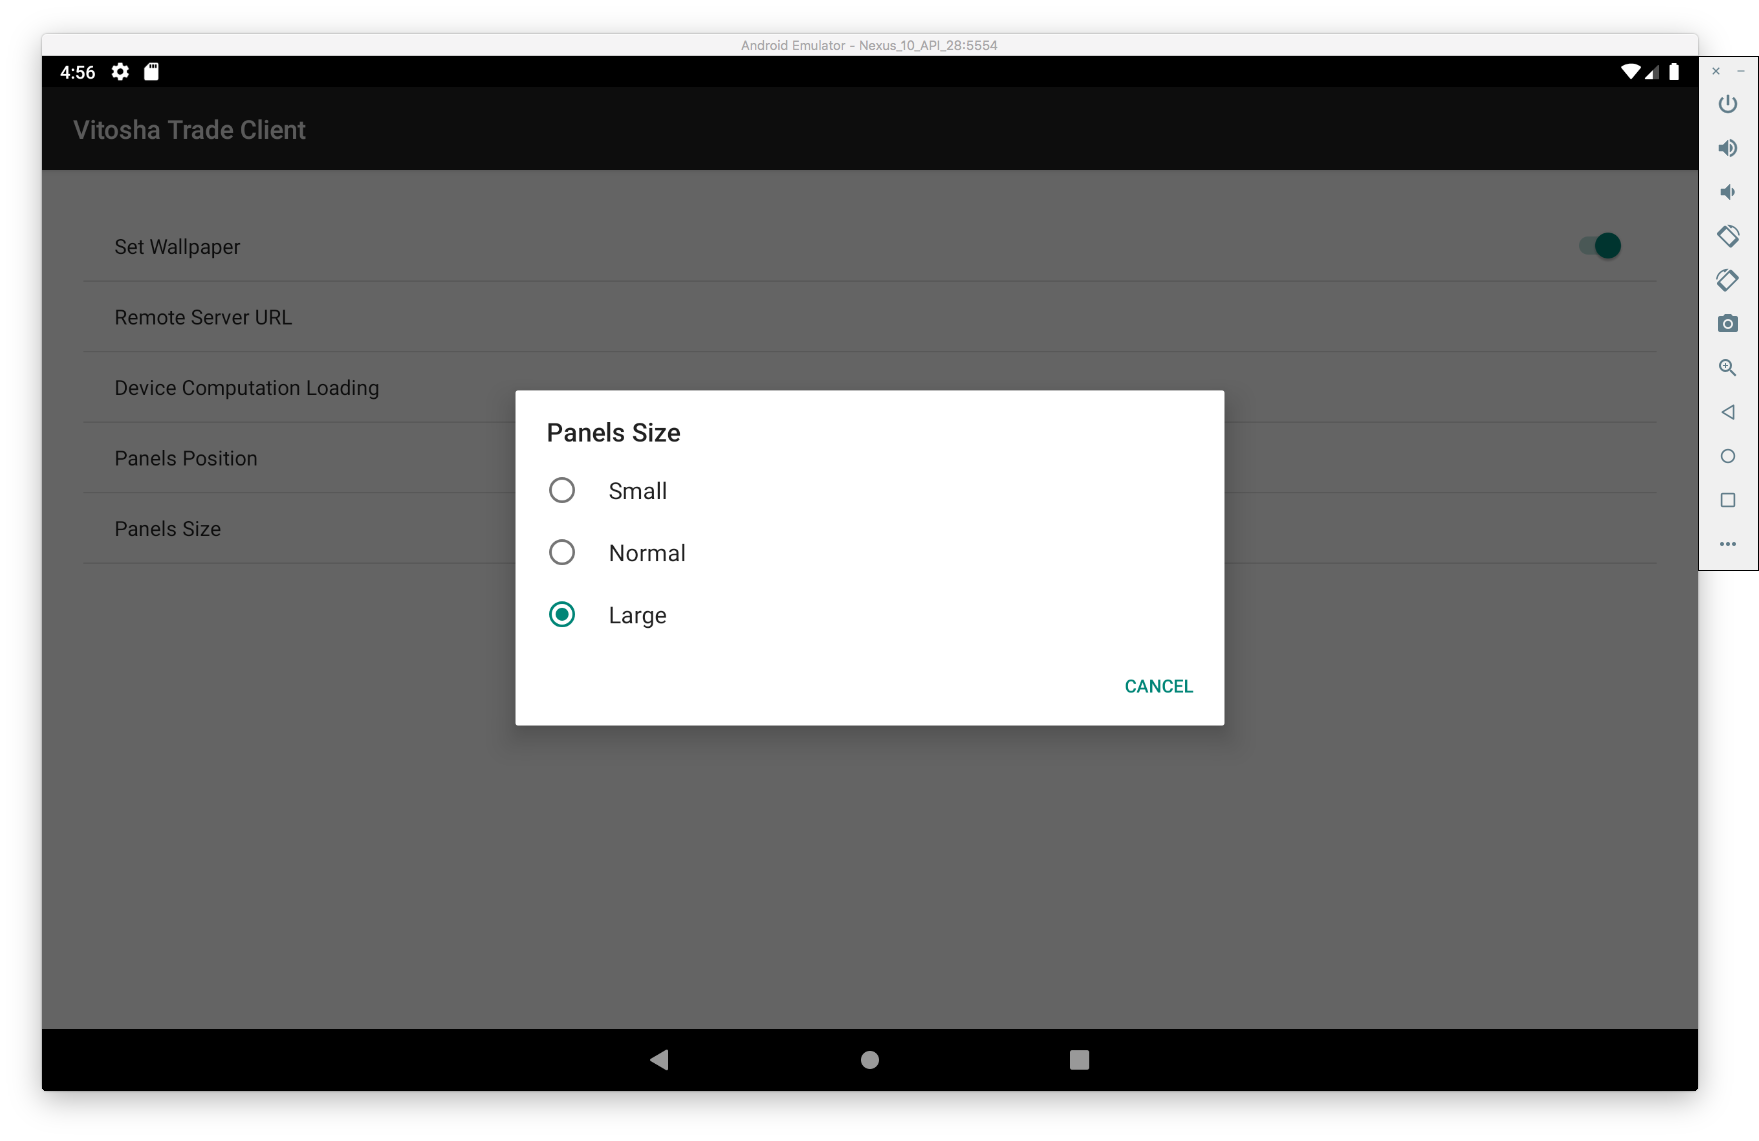
\includegraphics[width=0.8\linewidth]{fig0063.png}
  \caption{Размери на панелите за визуализация}
\label{fig0063}
\end{figure}

Графичният потребителски интерфейс, освен статична визуализация на междинни резултати, позволява и събиране на субективното мнение на потребителя. Това става с помощта на widget за гласуване (Фиг. \ref{fig0064}). Потребителят избира дали цената на определен актив ще се повиши или ще спадне. Целта е тази информация да се използва за разпределени изчисления по схемата човек-компютър. Всеки потребител има свое собствено мнение за движението на цената и това мнение най-често е интуитивно.  Компонентът за гласуване също има свой екран за настройки (Фиг. \ref{fig0065}).

\begin{figure}[H]
  \centering
  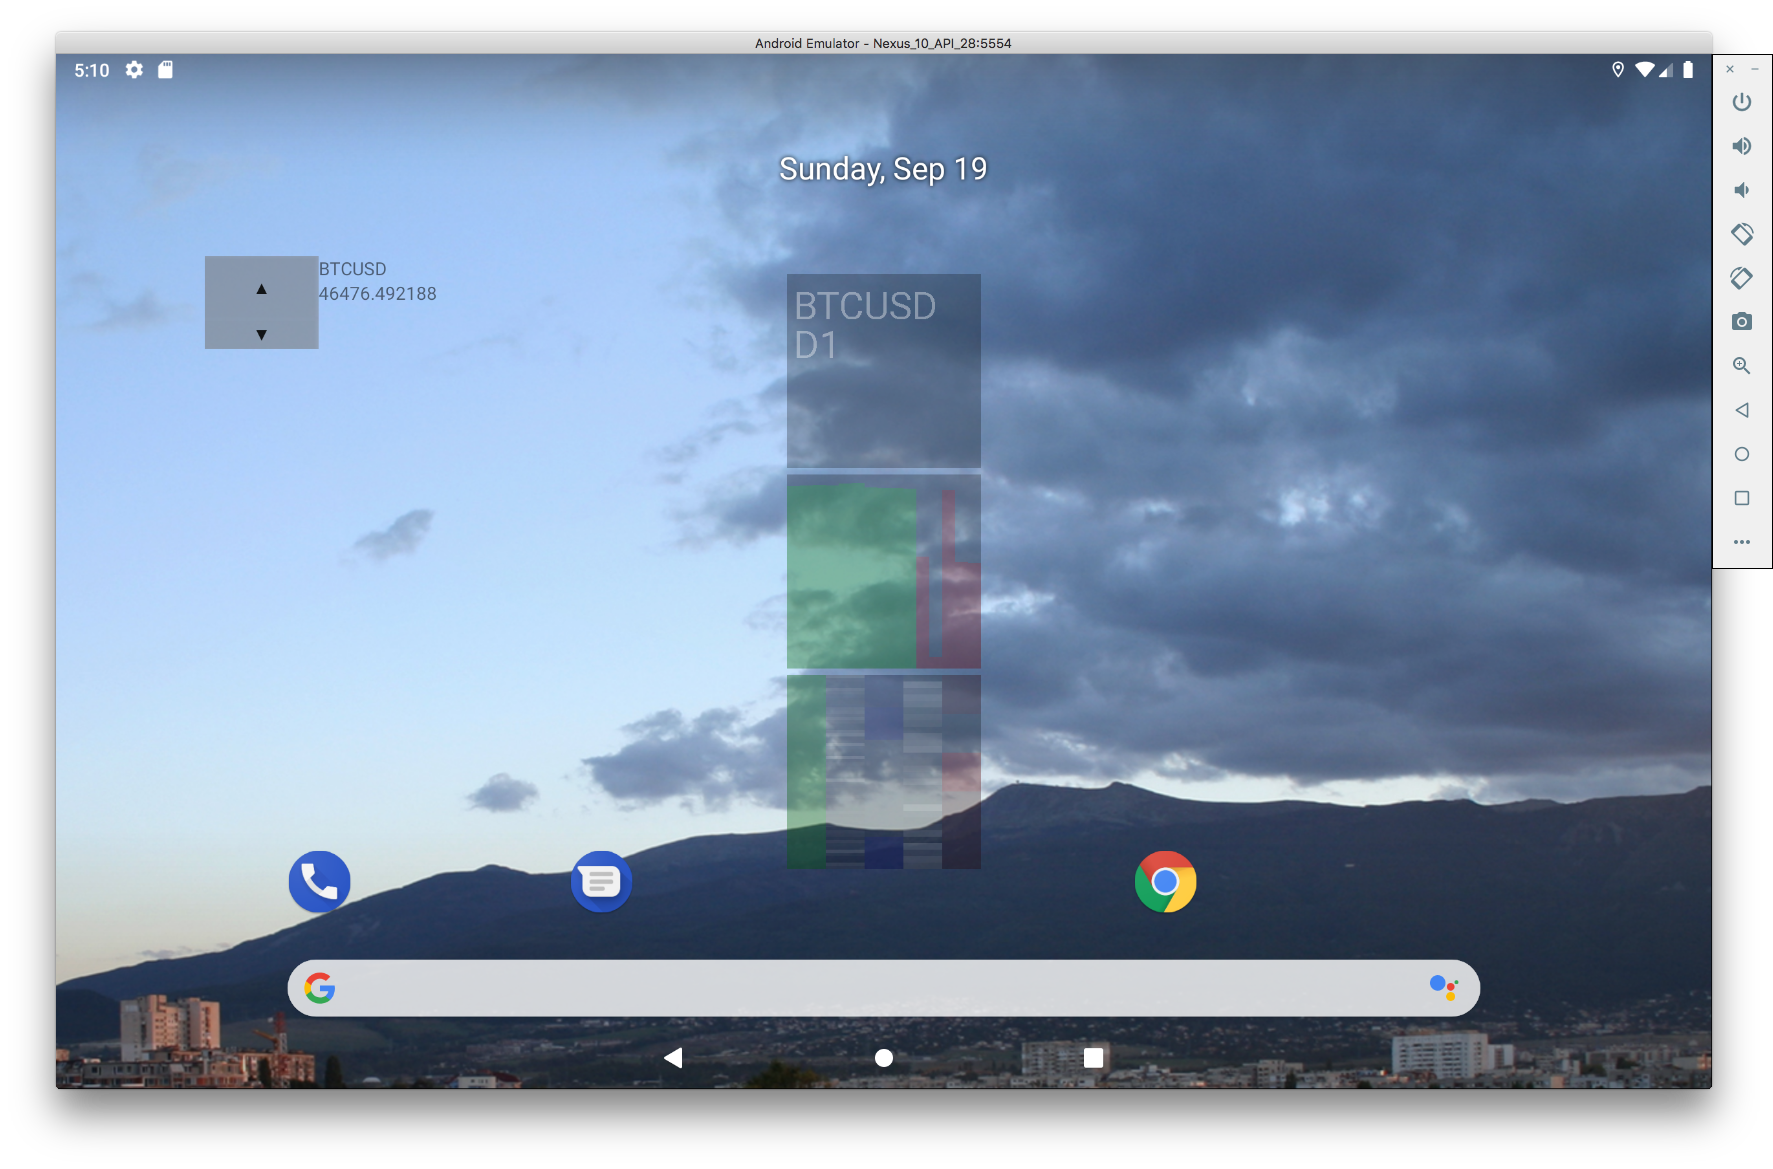
\includegraphics[width=0.8\linewidth]{fig0064.png}
  \caption{Компонент за гласуване}
\label{fig0064}
\end{figure}

При гласуване, в локалната SQLite база данни се записват точният час на гласуване, за коя валутна двойка е подаден гласът, посоката за промяна на цената, която потребителят е избрал и уникален идентификатор на потребителя. При наличие на Интернет свързаност, същата информация се изпраща и до отдалечения сървър. 

\begin{figure}[H]
  \centering
  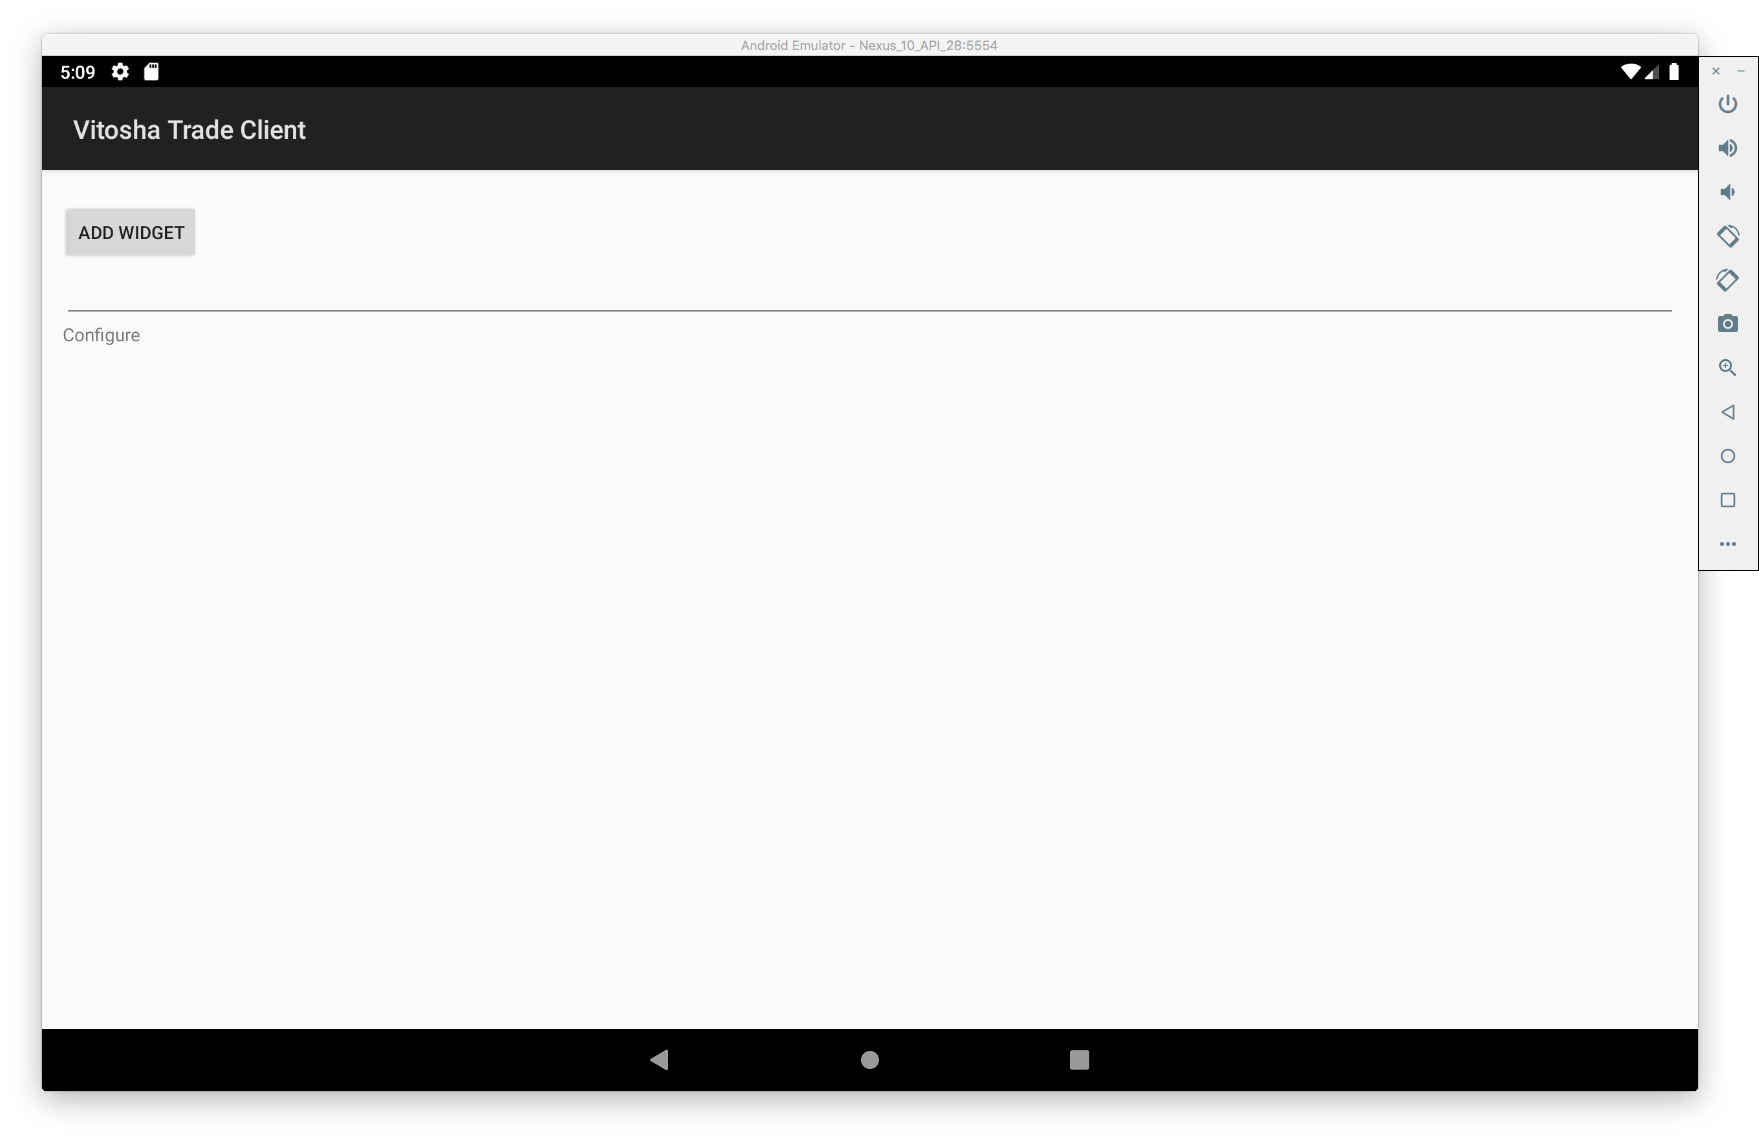
\includegraphics[width=0.8\linewidth]{fig0065.png}
  \caption{Настройки на компонента за гласуване}
\label{fig0065}
\end{figure}

Възможностите за съхраняване на информация в паметта на мобилното устройство, чрез SQLite е функционалност предоставена от самата операционна система Android. Поради тази причина, в модула за Android е добавен и помощен, междинен компонент за работа с релационната база данни. Терминът за такъв вид компоненти е Database Helper.

\subsection{Компоненти в модула за изчисление}

Изчислителният модул е организиран в два компонента – компонент за мрежова комуникация и компонент за обучение/прогнозиране (Фиг. \ref{fig0066}). Мрежовата комуникация е изнесена извън потребителския интерфейс, защото комуникацията с отдалечения сървър е необходима без значение дали приложението работи в Android OS средата или в терминалния прозорец на настолна компютърна конфигурация. 

\begin{figure}[H]
  \centering
  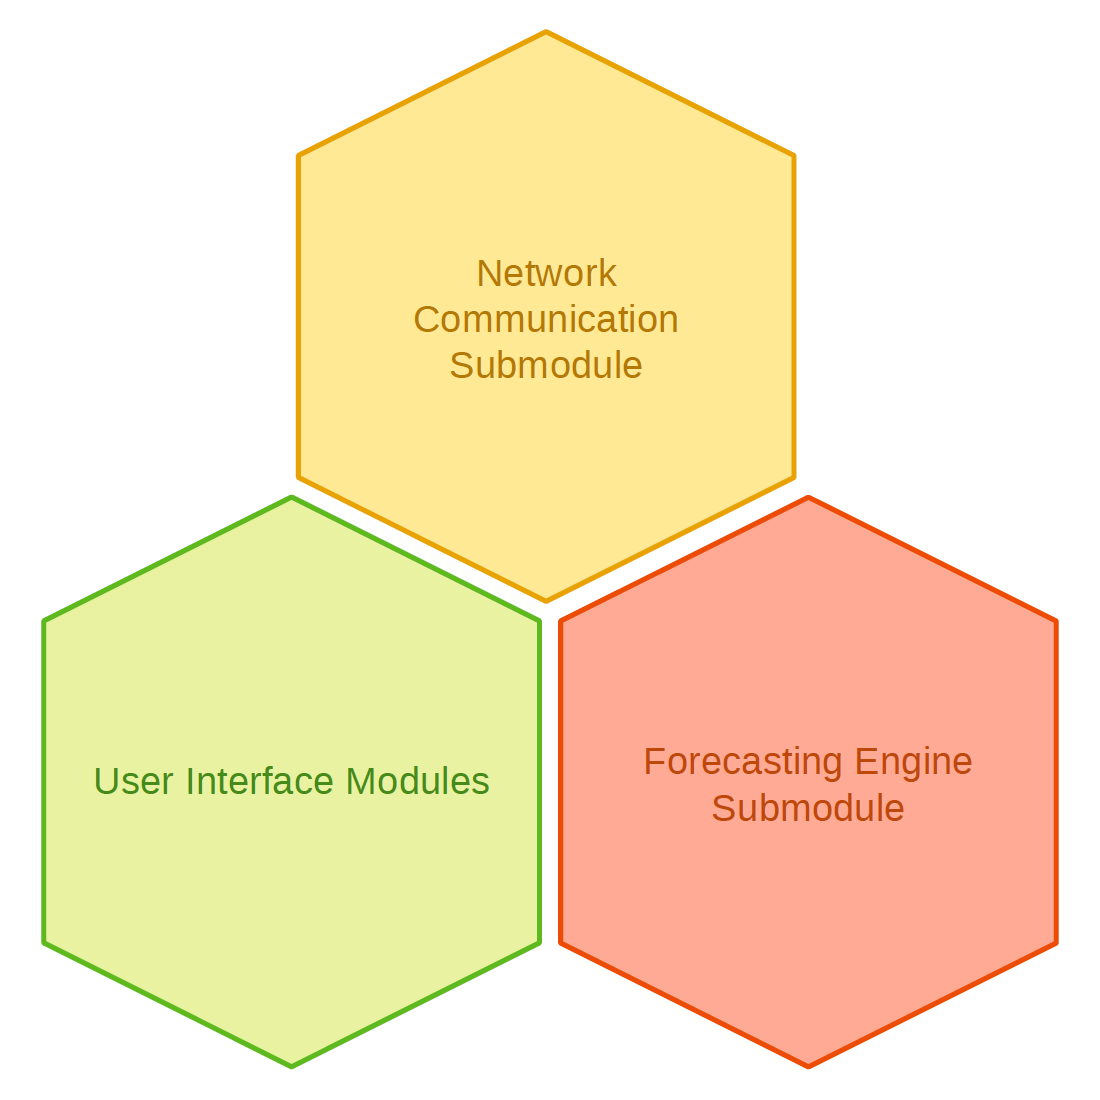
\includegraphics[width=0.8\linewidth]{fig0066.png}
  \caption{Структура на изчислителния модул}
\label{fig0066}
\end{figure}

Комуникацията с отдалечения сървър е организирана под формата на отделен Java клас, който изпълнява функцията на HTTP Helper (Фиг. \ref{fig0067}). Обменът на данните по HTTP протоколът е възможен благодарение на външна програмна библиотека (HttpClient for Android). Тъй като обменяните съобщения с отдалечения сървър са организирани под формата на JSON пакети, за обработката им се използва също външна библиотека (
JSON In Java).

\begin{figure}[H]
  \centering
  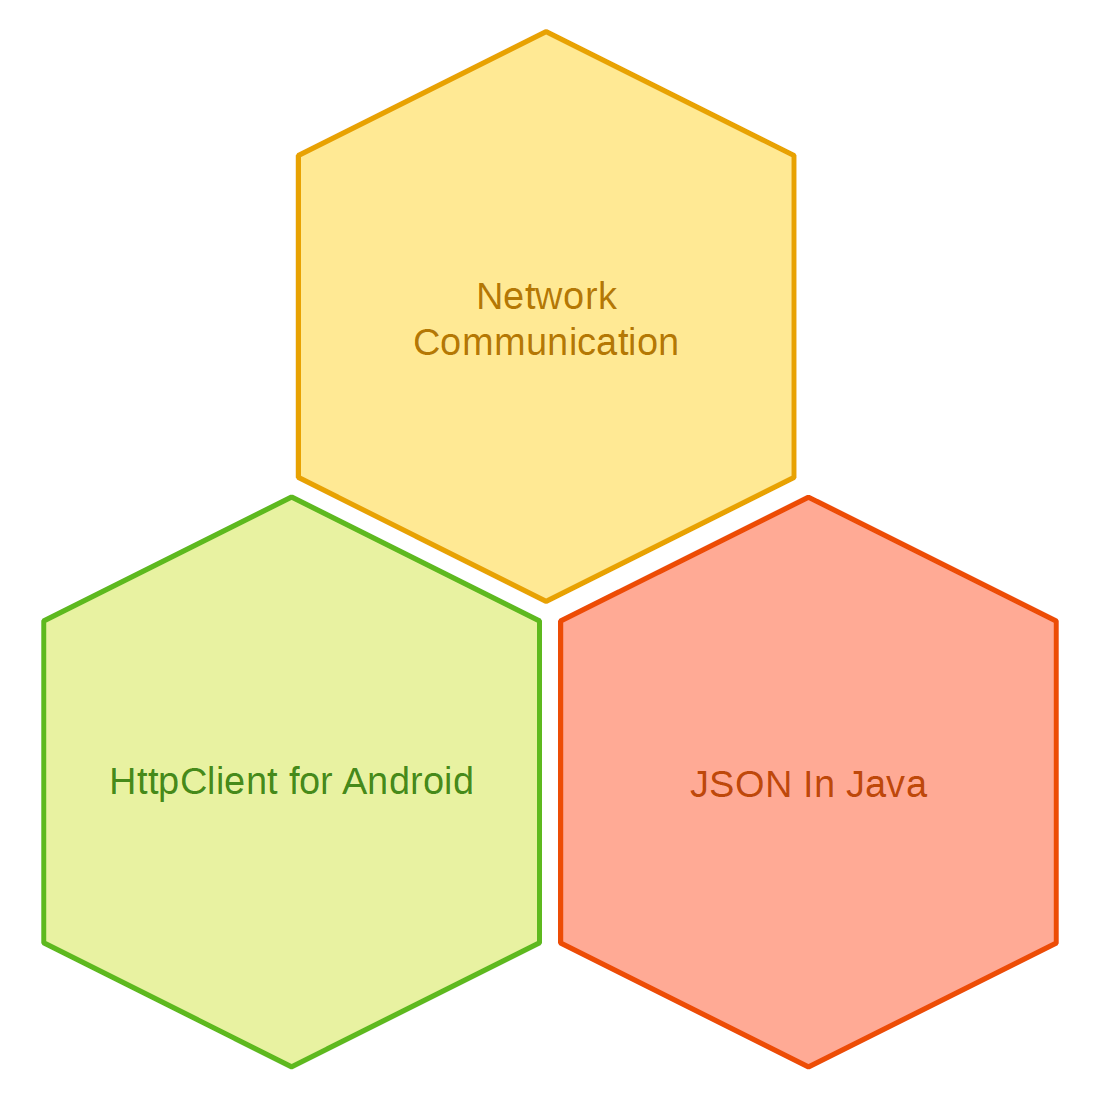
\includegraphics[width=0.8\linewidth]{fig0067.png}
  \caption{Организация на мрежовата комуникация}
\label{fig0067}
\end{figure}

Конструирането на изкуствената невронна мрежа, организацията на данните на входа и на изхода й, както и евристичните алгоритми за обучение са осъществени с помощта на външни програмни библиотеки. 

\begin{figure}[H]
  \centering
  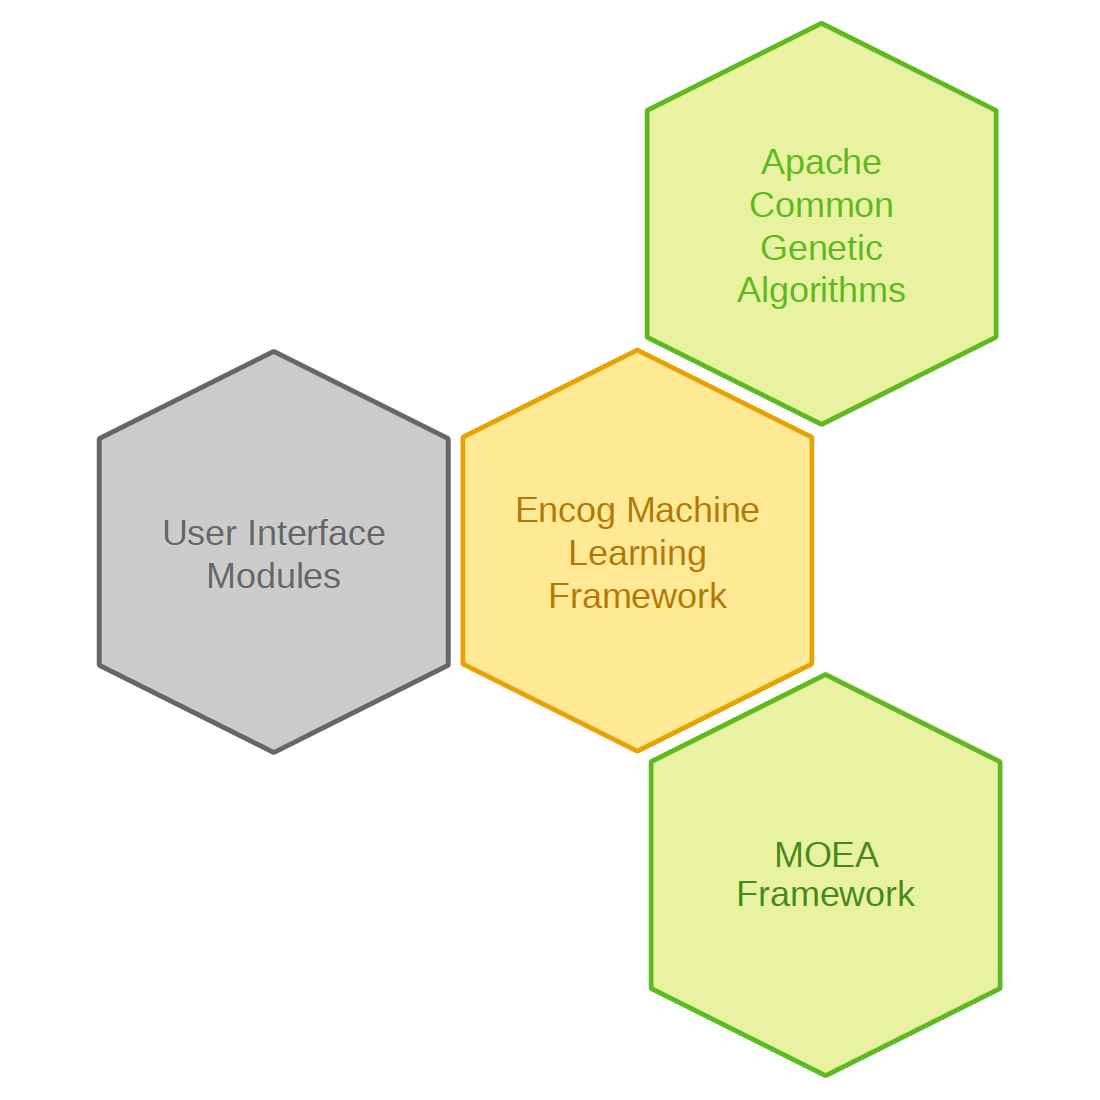
\includegraphics[width=0.8\linewidth]{fig0068.png}
  \caption{Организация на обучението/прогнозирането}
\label{fig0068}
\end{figure}

Изкуствената невронна мрежа се изгражда с помощта на библиотеката Encog Machine Learning Framework. В самата библиотека е реализирано обучение с обратно разпространение на грешката. Допълнително две библиотеки реализират глобална евристична оптимизация – Apache Common Genetic Algorithms и MOEA Framework.


